\documentclass[18pt, compress, aspectratio=169]{beamer}

% can be compiled by xelatex -shell-escape presentation.tex

\usetheme[usetitleprogressbar]{m}

\usepackage[utf8]{inputenc}
\usepackage[russian, english]{babel}
\usepackage{booktabs}
\usepackage[scale=2]{ccicons}
\usepackage{listings}
\usepackage{marvosym}
\usepackage{color}
\usepackage{xcolor}
\usepackage[document]{ragged2e}
\usepackage[export]{adjustbox}
\usepackage{fontawesome}
\usepackage{enumitem}
\usepackage{minted}
\usemintedstyle{tango}
%\usemintedstyle{monokai}

\usetikzlibrary{shapes,arrows,positioning}
\graphicspath{{images/}}
\newfontfamily{\FA}{FontAwesome}

\definecolor{check}{rgb}{0.1,2,0.3}
\definecolor{fail}{rgb}{2,0.1,0.1}
\definecolor{question}{rgb}{0.9,0.9,0.0}

\def\twitter{{\FA \faTwitter}}
\def\github{{\FA \faGithubSign}}
\def\email{{\FA \faEnvelope}}
\def\check{\textcolor{check}{\FA \faCheck}}
\def\fail{\textcolor{fail}{\FA \faRemove}}
\def\question{\textcolor{question}{\FA \faSearch}}

\renewcommand{\ttdefault}{pcr}
\newfontfamily{\ttfamily}{Fira Code}
\makeatletter
\newcommand\HUGE{\@setfontsize\Huge{38}{47}}
\makeatother

\definecolor{links}{HTML}{0099FF}
\hypersetup{colorlinks, linkcolor=, urlcolor=links}

\setbeamerfont{section title}{family=\Book, size=\Huge, shape=\normalfont}
\setbeamerfont{frametitle}{family=\Book, size=\large, shape=\normalfont}
\setbeamerfont{title}{family=\Book, size=\HUGE, shape=\normalfont}
\setbeamerfont{subtitle}{size=\Huge}

\title{FP in Python/JS}
\date{\today}
\institute{}

\begin{document}
\fontsize{19pt}{20}\selectfont
\maketitle

\section{}

\begin{frame}
    \frametitle{Why?}
    \vspace{-25pt}
    \begin{figure}
        
\includegraphics[width=0.8\textwidth,center]{first_option.png}
    \end{figure}
\end{frame}

\begin{frame}
    \frametitle{Why?}
    \vspace{-25pt}
    \begin{figure}
        
\includegraphics[width=0.8\textwidth,center]{second_option.png}
    \end{figure}
\end{frame}

\begin{frame}[fragile]
    \frametitle{Why?}
    \begin{itemize}[label={\MVRightarrow}]
        \item FP is a paradigm, not a language feature
        \item Python is a multi-paradigm language, that allows to wright in functional style
        \item It's possible to use advantages of FP today
    \end{itemize}
\end{frame}

\begin{frame}
    \frametitle{Pros and cons}
    \vspace{-20pt}
    \begin{columns}[T,onlytextwidth]
    \column{0.5\textwidth}
        \begin{itemize}[label={\MVRightarrow}]
            \item <+->Logic is separated from data \check
            \item <+->Modularity, testability \check
            \item <+->Parallelization \check
        \end{itemize}

    \column{0.45\textwidth}
        \begin{itemize}[label={\MVRightarrow}]
            \item <+->Difficult \fail
            \item <+->Scary \fail
            \item <+->Developers? \fail
        \end{itemize}
    \end{columns}
\end{frame}

\begin{frame}[fragile]
    \frametitle{Кто?}
    \begin{itemize}[label={\MVRightarrow}]
        \item postgrest
        \item pandoc
        \item elm-compiler
        \item purescript
        \item aura (arch linux package manager)
    \end{itemize}
\end{frame}

\section{Introduction in FP}

\begin{frame}[fragile]
    \frametitle{Terms and definitions}
    \begin{itemize}[label={\MVRightarrow}]
        \item Immutability
        \item Pure functions and side effects
        \item Higher-order functions
        \item Monads (?)
        \item Abstract Data Type (ADT)
    \end{itemize}
\end{frame}

\begin{frame}
    \frametitle{Immutability, persistency}
    \vspace{-20pt}
    \begin{figure}
        
\includegraphics[width=1.0\textwidth,center]{Vault_Boy_text.png}
    \end{figure}
\end{frame}

\begin{frame}
    \frametitle{Pure functions and side effects}
    \vspace{-25pt}
    \begin{figure}
        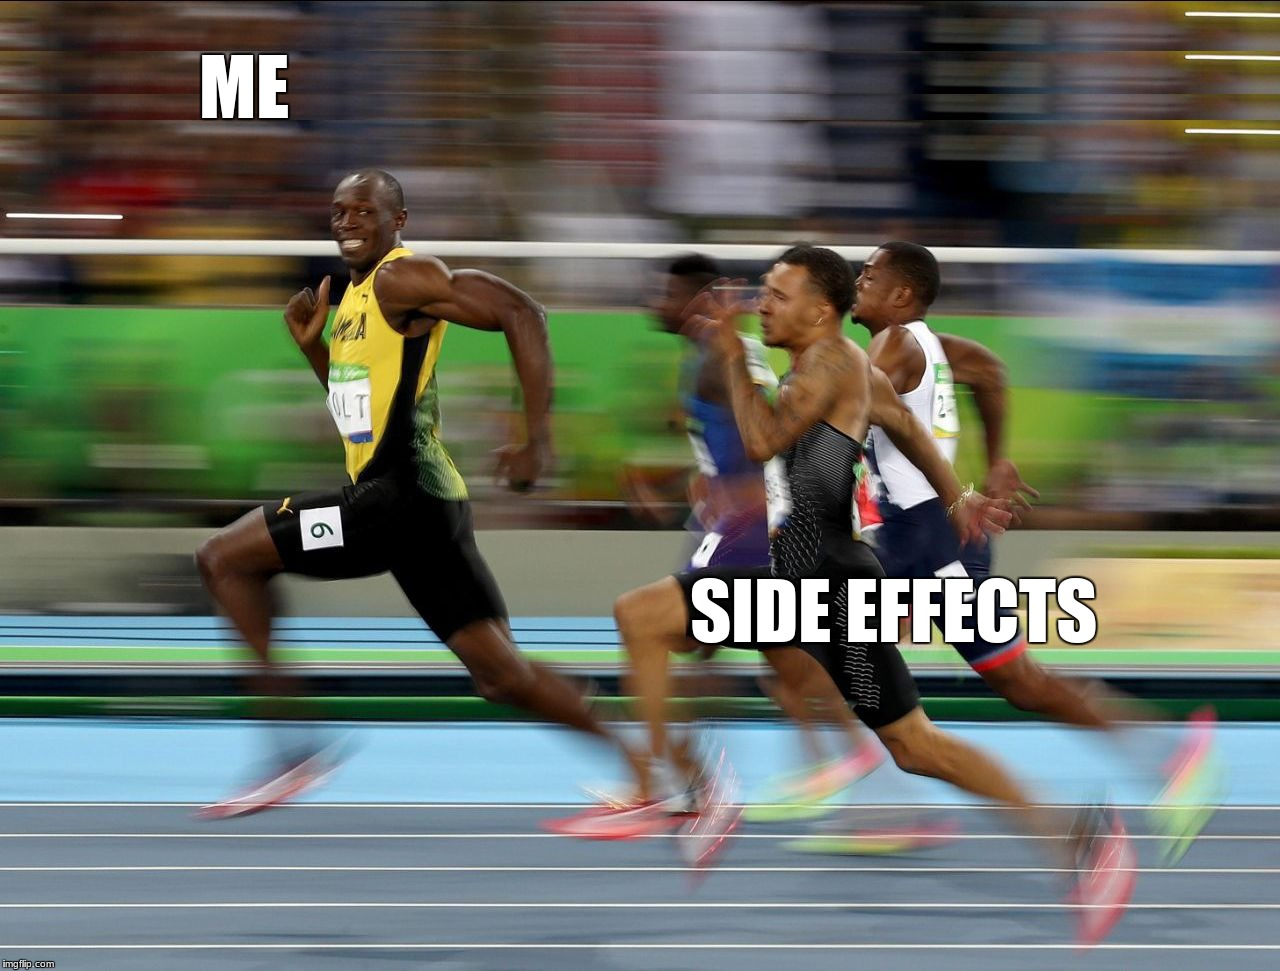
\includegraphics[width=0.7\textwidth,center]{side_effect.jpg}
    \end{figure}
\end{frame}

\begin{frame}
    \frametitle{Higher-order functions and function composition}
    \vspace{-25pt}
    \begin{figure}
        
\includegraphics[width=0.53\textwidth,center]{function_composition.jpg}
    \end{figure}
\end{frame}

\begin{frame}
    \frametitle{Monads, ADT}
    \vspace{-20pt}
    \begin{figure}
        
\includegraphics[width=0.5\textwidth,center]{squirells.png}
    \end{figure}
\end{frame}

\section{FP support in Python}

\begin{frame}
    \frametitle{What's available}
    \vspace{-25pt}
    \begin{itemize}[label={\MVRightarrow}]
        \item <+->Immutable data types:
            \begin{itemize}
                \item string
                \item tuple/namedtuple
                \item fronzenset
            \end{itemize}
        \item <+->Higher-order functions
        \item <+->List comprehension
        \item <+->Generators
        \item <+->itertools
        \item <+->functools
    \end{itemize}
\end{frame}

\begin{frame}
    \frametitle{What's missing}
    \begin{overlayarea}{\textwidth}{.8\textheight}
    \begin{itemize}[label={\MVRightarrow}]
        \item <1->Tail recursion optimization \fail
        \item <2->Pure functions \fail
        \item <3|only@3>Pattern matching \alt<3>{\fail}{\question}
        \item <4->Pattern matching \alt<3>{\fail}{\question}
        \item <5|only@5>Automatic currying \alt<5>{\fail}{\question}
        \item <6->Automatic currying \alt<5>{\fail}{\question}
        \item <7|only@7>Monads \alt<7>{\fail}{\question}
        \item <8->Monads \alt<7>{\fail}{\question}
        \item <9|only@9>ADT \alt<9>{\fail}{\question}
        \item <10->ADT \alt<9>{\fail}{\question}
    \end{itemize}
    \end{overlayarea}
\end{frame}

\section{FP support in JS/Coffeescript}

\begin{frame}
    \frametitle{What's available}
    \vspace{-25pt}
    \begin{itemize}[label={\MVRightarrow}]
        \item <+->Immutable data types:
            \begin{itemize}
                \item Object.freeze
            \end{itemize}
        \item <+->Higher-order functions
        \item <+->List comprehension
        \item <+->lodash/underscore
    \end{itemize}
\end{frame}

\begin{frame}
    \frametitle{What's missing}
    \begin{overlayarea}{\textwidth}{.8\textheight}
    \begin{itemize}[label={\MVRightarrow}]
        \item <1->Most immutable data types \fail
        \item <1->Tail recursion optimization \fail
        \item <2->Pure functions \fail
        \item <3|only@3>Pattern matching \alt<3>{\fail}{\question}
        \item <4->Pattern matching \alt<3>{\fail}{\question}
        \item <5|only@5>Automatic currying \alt<5>{\fail}{\question}
        \item <6->Automatic currying \alt<5>{\fail}{\question}
        \item <7|only@7>Monads \alt<7>{\fail}{\question}
        \item <8->Monads \alt<7>{\fail}{\question}
        \item <9|only@9>ADT \alt<9>{\fail}{\question}
        \item <10->ADT \alt<9>{\fail}{\question}
    \end{itemize}
    \end{overlayarea}
\end{frame}

\begin{frame}
    \frametitle{Strategies}
    \begin{itemize}[label={\MVRightarrow}]
        \item Pure Python/JS
        \item Utility functions
        \item Third party libraries
    \end{itemize}
\end{frame}

\section{Examples (py2)}

\setbeamercolor{background canvas}{bg=white}
\begin{frame}[fragile]
    \setbeamertemplate{section page}
    \frametitle{}
    \begin{center}
    \inputminted[
        fontsize=\large,
        %bgcolor=black,
    ]{python}{examples/immutable.py}
    \inputminted[
        fontsize=\large,
        %bgcolor=black,
    ]{coffeescript}{examples/immutable.coffee}
    \end{center}
\end{frame}

\begin{frame}[fragile]
    \setbeamertemplate{section page}
    \frametitle{}
    \begin{center}
    \inputminted[
        fontsize=\large,
    ]{python}{examples/list_comprehension.py}
    \end{center}
\end{frame}

\begin{frame}[fragile]
    \setbeamertemplate{section page}
    \frametitle{}
    \begin{center}
    \inputminted[
        fontsize=\large,
    ]{coffeescript}{examples/list_comprehension.coffee}
    \end{center}
\end{frame}

\begin{frame}[fragile]
    \setbeamertemplate{section page}
    \frametitle{}
    \begin{center}
    \inputminted[
        fontsize=\large,
    ]{haskell}{examples/list_comprehension.hs}
    \end{center}
\end{frame}

\begin{frame}[fragile]
    \setbeamertemplate{section page}
    \frametitle{}
    \begin{center}
    \inputminted[
        fontsize=\large,
    ]{python}{examples/generators.py}
    \end{center}
\end{frame}

\begin{frame}[fragile]
    \setbeamertemplate{section page}
    \frametitle{}
    \begin{center}
    \inputminted[
        fontsize=\large,
    ]{javascript}{examples/generators.js}
    \end{center}
\end{frame}

\begin{frame}[fragile]
    \setbeamertemplate{section page}
    \frametitle{}
    \begin{center}
    \inputminted[
        fontsize=\large,
    ]{javascript}{examples/wu.js}
    \end{center}
\end{frame}

\begin{frame}[fragile]
    \setbeamertemplate{section page}
    \frametitle{}
    \begin{center}
    \inputminted[
        fontsize=\large,
    ]{python}{examples/maybe_example.py}
    \end{center}
\end{frame}

\begin{frame}[fragile]
    \setbeamertemplate{section page}
    \frametitle{}
    \begin{center}
        \begin{figure}
            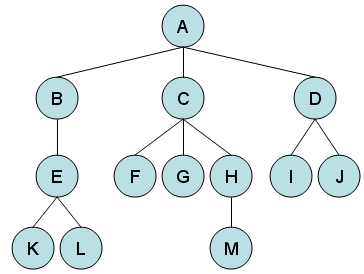
\includegraphics[width=0.5\textwidth,center]{tree.png}
        \end{figure}
    \end{center}
\end{frame}

\begin{frame}[fragile]
    \setbeamertemplate{section page}
    \frametitle{}
    \begin{center}
    \inputminted[
        fontsize=\large,
    ]{python}{examples/recursion_1.py}
    \end{center}
\end{frame}

\begin{frame}[fragile]
    \setbeamertemplate{section page}
    \frametitle{}
    \begin{center}
    \inputminted[
        fontsize=\large,
    ]{python}{examples/recursion_2.py}
    \end{center}
\end{frame}

\begin{frame}[fragile]
    \setbeamertemplate{section page}
    \frametitle{}
    \begin{center}
    \inputminted[
        fontsize=\large,
    ]{python}{examples/recursion_fp.py}
    \end{center}
\end{frame}

\begin{frame}[fragile]
    \setbeamertemplate{section page}
    \frametitle{}
    \begin{center}
    \inputminted[
        fontsize=\large,
    ]{python}{examples/curry_example1.py}
    \end{center}
\end{frame}

\begin{frame}[fragile]
    \setbeamertemplate{section page}
    \frametitle{}
    \begin{center}
    \inputminted[
        fontsize=\large,
    ]{python}{examples/curry_example2.py}
    \end{center}
\end{frame}

\begin{frame}[fragile]
    \setbeamertemplate{section page}
    \frametitle{}
    \begin{center}
    \inputminted[
        fontsize=\large,
    ]{python}{examples/example1.py}
    \end{center}
\end{frame}

\begin{frame}[fragile]
    \setbeamertemplate{section page}
    \frametitle{}
    \begin{center}
    \inputminted[
        fontsize=\large,
    ]{python}{examples/example2.py}
    \end{center}
\end{frame}

\begin{frame}[fragile]
    \setbeamertemplate{section page}
    \frametitle{}
    \begin{center}
    \inputminted[
        fontsize=\large,
    ]{python}{examples/example3.py}
    \end{center}
\end{frame}

\begin{frame}[fragile]
    \setbeamertemplate{section page}
    \frametitle{}
    \begin{center}
    \inputminted[
        fontsize=\large,
    ]{python}{examples/example4.py}
    \end{center}
\end{frame}
\note{http://programmers.stackexchange.com/questions/150837/maybe-monad-vs-exceptions}

\begin{frame}[fragile]
    \setbeamertemplate{section page}
    \frametitle{}
    \begin{center}
    \inputminted[
        fontsize=\large,
    ]{coffeescript}{examples/pattern_matching.coffee}
    \end{center}
\end{frame}

\begin{frame}[fragile]
    \setbeamertemplate{section page}
    \frametitle{}
    \begin{center}
    \inputminted[
        fontsize=\small,
    ]{coffeescript}{examples/pattern_matching_fp.coffee}
    \end{center}
\end{frame}

\begin{frame}
    \vspace{7pt}
    \begin{figure}
        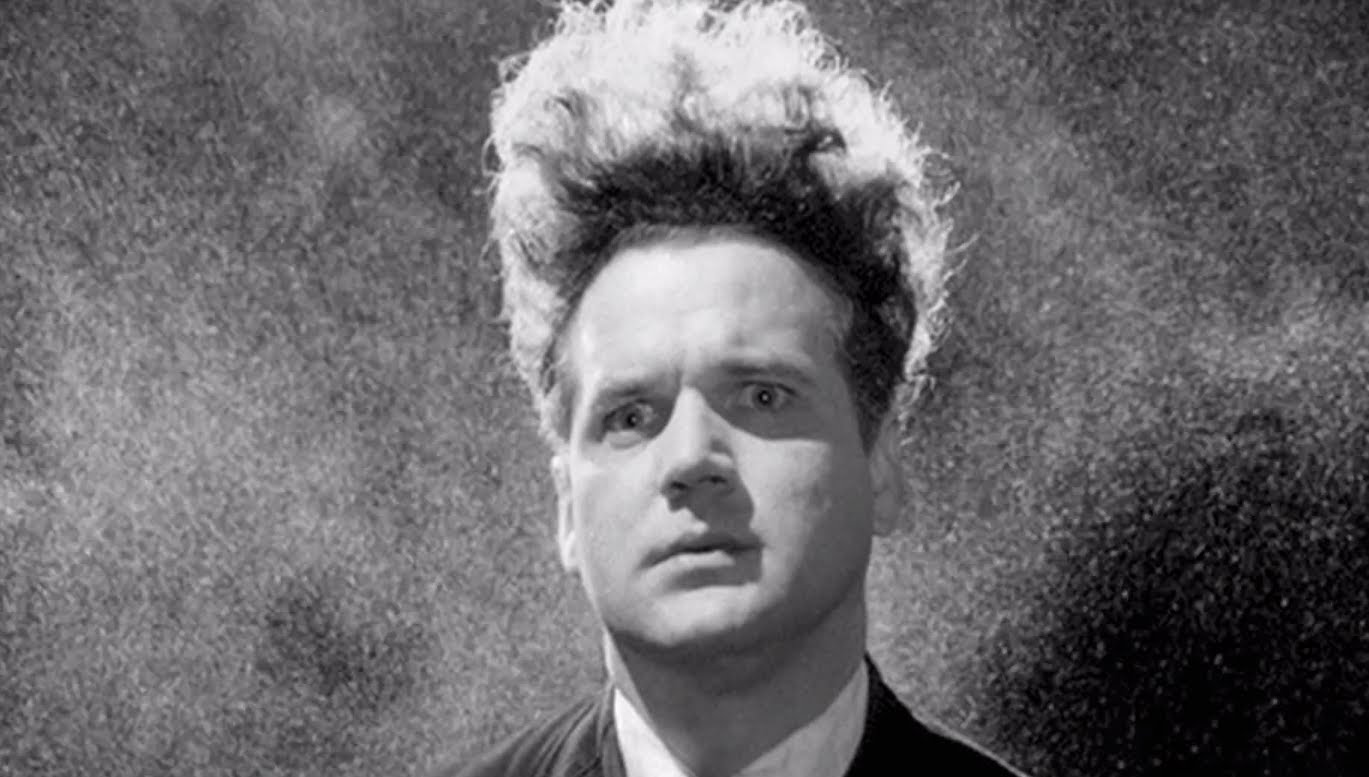
\includegraphics[width=1.0\textwidth,center]{mindblown.jpg}
    \end{figure}
\end{frame}

\setbeamercolor{background canvas}{bg=palette primary.bg}

\section{Libraries}

\fontsize{15pt}{16}\selectfont
\begin{frame}
    \frametitle{List of FP libraries for Python}
    \vspace{-35pt}
    \begin{columns}[T,onlytextwidth]
        \column{0.5\textwidth}
        \begin{itemize}[label={\MVRightarrow}]
            \item PyFunctional
            \item toolz
            \item adt
            \item Coconat
            \item pyrsistent
            \item funcy
            \item effect
            \item hask
            \item fn.py
            \item PyMonad
        \end{itemize}

        \column{0.5\textwidth}
        \begin{itemize}[label={}]
            \item \href{github.com/EntilZha/PyFunctional}{EntilZha/PyFunctional}
            \item \href{github.com/pytoolz/toolz}{pytoolz/toolz}
            \item \href{github.com/llllllllll/adt}{llllllllll/adt}
            \item \href{github.com/evhub/coconut}{evhub/coconut}
            \item \href{github.com/Suor/funcy}{Suor/funcy}
            \item \href{github.com/tobgu/pyrsistent}{tobgu/pyrsistent}
            \item \href{github.com/python-effect/effect}{python-effect/effect}
            \item \href{github.com/billpmurphy/hask}{billpmurphy/hask}
            \item \href{github.com/kachayev/fn.py}{kachayev/fn.py}
            \item \href{github.com/fnl/pymonad}{fnl/pymonad}
        \end{itemize}

    \end{columns}
\end{frame}
\fontsize{19pt}{20}\selectfont
%https://www.npmjs.com/package/adt
%https://www.npmjs.com/package/adt-simple
%https://www.npmjs.com/package/akh.maybe
%https://www.npmjs.com/package/coffee-monad
%https://www.npmjs.com/package/curry
%https://www.npmjs.com/package/auto-curry
%https://www.npmjs.com/package/match-when
%https://www.npmjs.com/package/match-js

\begin{frame}
    \frametitle{Why?}
    \vspace{-25pt}
    \begin{itemize}[label={\MVRightarrow}]
        \item A lot of functions
        \item Decorator @curry
        \item Persistent data types
        \item Nice syntax for function composition
        \item Decorator to bypass tail recursion optimization
        \item Monads and ADT
    \end{itemize}
\end{frame}

\plain{Questions?}

\end{document}
